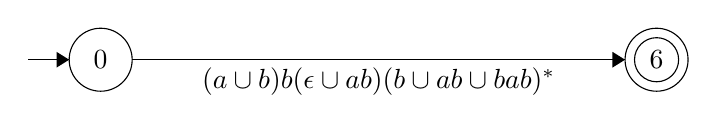
\begin{tikzpicture}[scale=0.2]
    \tikzstyle{every node}+=[inner sep=0pt]
    \draw [black] (4.8,-2.2) circle (2);
    \draw (4.8,-2.2) node {$0$};
    \draw [black] (40.1,-2.2) circle (2);
    \draw (40.1,-2.2) node {$6$};
    \draw [black] (40.1,-2.2) circle (1.4);
    \draw [black] (0.2,-2.2) -- (2.8,-2.2);
    \fill [black] (2.8,-2.2) -- (2,-1.7) -- (2,-2.7);
    \draw [black] (6.8,-2.2) -- (38.1,-2.2);
    \fill [black] (38.1,-2.2) -- (37.3,-1.7) -- (37.3,-2.7);
    \draw (22.45,-2.7) node [below] {$(a\cup b)b(\epsilon\cup ab)(b\cup ab \cup bab)^*$};
    \end{tikzpicture}